\section*{Lernskript: Eigengesichter}
Historisch gesehen war die Methode der Eigengesichter das erste durch Computer automatisierbare Verfahren zur Gesichtserkennung.
Das Fundament dazu wurde 1987 durch Sirovich and Kirby entwickelt \cite{SirovichKirby1987}.
In ihrer Arbeit verwendeten Sie bereits den Begriff \textit{eigenpictures}.
Sie zeigten auf, wie man Fotos von Gesichtern geeignet durch Begriffe der linearen Algebra beschreiben kann.
Damit war der Weg frei um die mächtige Maschinerie der Mathematik, insbesondere der linearen Algebra und der Statistik, auf Fotos anzuwenden.
Dies geschah schon kurz darauf, nämlich 1991, durch Turk und Pentland \cite{Turk1991}.
Sie verwendeten bereits den Begriff \textit{eigenfaces} und beschrieben das Verfahren zur Gesichtserkennung, welches auch wir implementieren werden.
Modernere Methoden wie zum Beispiel \textit{DeepFace} von Facebook funktionieren allerdings viel besser als unsere rudimentäre Methode und sind so gut wie echte Menschen bei der Gesichtserkennung \cite{Taigman2014}.
Ein Vergleich der (heutzutage) besten Methoden findet man zum Beispiel hier \cite{Taskiran2020}.

Alle solchen Programme, auch die modernsten, verwenden eine \textit{Datenbank} von Bildern von Gesichtern, deren Identität bereits bekannt ist.
Man hat also eine gewisse Anzahl von Personen.
Jeder einzelnen Person sind mehrere Bilder zugeordnet, nämlich die Bilder, welche das Gesicht eben dieser Person zeigen.
Man kann sich das als Unterteilung in verschiedene Klassen vorstellen: Zu jeder Person gehört eine Klasse und jede Klasse enthält eine Menge von Bildern.
Dies ist in Abbildung~\ref{fig:database} veranschaulicht.
\begin{figure}[ht]
	\centering
	\begin{tabular}{l m{2cm} m{2cm} m{2cm} m{2cm} c}
		\textbf{Klasse (Person)} & \textbf{Bild 1} & \textbf{Bild 2} & \textbf{Bild 3} & \textbf{Bild 4} & $\cdots$ \\ \hline
		Adam Sandler & 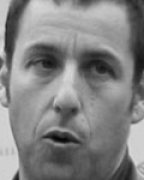
\includegraphics[width=0.1\textwidth]{images/intro/class0_0} &
		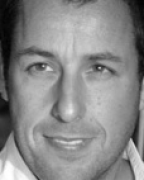
\includegraphics[width=0.1\textwidth]{images/intro/class0_1} & 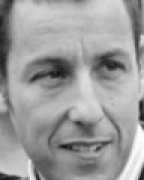
\includegraphics[width=0.1\textwidth]{images/intro/class0_2} & 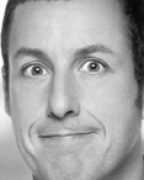
\includegraphics[width=0.1\textwidth]{images/intro/class0_3} & $\cdots$ \\ \hline
		Emma Watson & 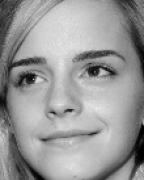
\includegraphics[width=0.1\textwidth]{images/intro/class1_0} &
		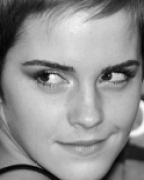
\includegraphics[width=0.1\textwidth]{images/intro/class1_1} & 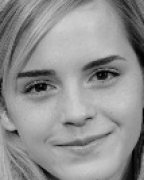
\includegraphics[width=0.1\textwidth]{images/intro/class1_2} & 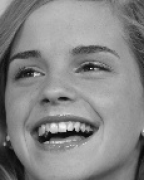
\includegraphics[width=0.1\textwidth]{images/intro/class1_3} & $\cdots$ \\ \hline
		Natalie Portman & 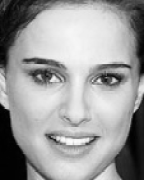
\includegraphics[width=0.1\textwidth]{images/intro/class2_0} & 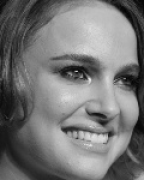
\includegraphics[width=0.1\textwidth]{images/intro/class2_1} & 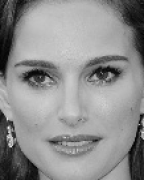
\includegraphics[width=0.1\textwidth]{images/intro/class2_2} & 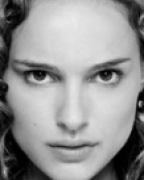
\includegraphics[width=0.1\textwidth]{images/intro/class2_3} & $\cdots$ \\ \hline
		$\qquad\qquad\vdots$ & $\qquad\vdots$ & $\qquad\vdots$ & $\qquad\vdots$ & $\qquad\vdots$ & $\ddots$ \\
	\end{tabular}
	\caption{Visualisierung einer Datenbank von Bildern von Gesichtern.}
	\label{fig:database}
\end{figure}
Aus dieser Datenbank \glqq{}lernt\grqq{} das Programm, neue Bilder zu klassifizieren, also den Personen aus der Datenbank zuzuordnen.
Das Wort \glqq{}neu\grqq{} bedeutet hier, dass dieses Bild nicht notwendigerweise in der Datenbank enthalten ist.
Die Person auf dem Bild muss aber in der Datenbank sein!
Würde die Datenbank in Abbildung~\ref{fig:database} wirklich nur diese drei Personen enthalten, so könnte man zum Beispiel kein Bild von Brad Pitt korrekt klassifizieren, auch wenn eine noch so gute Methode verwendet wird.
Die Datenbank und die Methode der Gesichtserkennung sind unabhängig voneinander.
Das heisst einerseits, aus der selben Datenbank können verschiedene Methoden lernen.
Andererseits kann ein und die selbe Methode verschiedene Datenbanken nutzen.
Wie gut die Gesichtserkennung am Schluss funktioniert hängt nicht nur von der Methode selbst ab, sondern auch von der Datenbank, welche diese verwendet.
Grundsätzlich gilt, dass jede Methode umso besser funktioniert, je mehr Bilder pro Person in der Datenbank gespeichert sind, die sie verwendet.
Mit \glqq{}gut funktionieren\grqq{} ist gemeint, dass neue Bilder mit hoher Wahrscheinlichkeit richtig klassifiziert werden.

Die in Abbildung~\ref{fig:database} gezeigten Bilder stammen aus einer Datenbank von über 10'000 Bildern von über 100 berühmten Persönlichkeiten \cite{Chen14}.
Die Bilder sind alle schwarz-weiss und zeigen lediglich die Gesichter der Personen.
Genau diese Datenbank werden wir auch für alle nachfolgenden Kapitel verwenden \textcolor{green}{(Link zur Datenbank folgt)}.
Allerdings kann auch eine andere Datenbank verwendet werden, sofern sie in das richtige Format gebracht wird \textcolor{green}{(Kapitel dazu folgt)}.

Das Grundgerüst eines Programms zur Gesichtserkennung in Python steht uns schon zur Verfügung.
Wir werden dieses in den folgenden Kapiteln zu einem voll funktionsfähigen Programm erweitern.
Der gesamte Code befindet sich im Anhang \textcolor{green}{(folgt)} und kann unter folgendem Link heruntergeladen werden \textcolor{green}{(Link zum Code folgt)}.